\par{Host code calls \emph{kernel} code multiple times based on the 
    number of global \emph{work items} declared and the number of vertices 
    on the surface of the selected bio molecule. There are 30 arguments 
    passed to the \emph{kernels}, with 16 of these being 
    \emph{\_\_global CL\_MEM\_READ\_ONLY}
    buffers and 1 being \emph{\_\_global CL\_MEM\_READ\_WRITE} buffer 
    for the final output. Pseudo code of the host is shown in listing 
    \ref{nbody_host}.}

\lstinputlisting[float,caption={Nbody host pseudo code.},label={nbody_host}, 
                style=customc]
                {/Users/lalanne/MyCode/GitHubProjects/OpenCLNotes/src/code/nbody_host.c}

\par{Every \emph{work item} in OpenCL is an implementation of the \emph{kernel} code. 
    Hence each \emph{work item} does a single step n body calculation. 
    i.e. Each \emph{work item} is working on the total electrostatic 
    potential on a vertex due to the atoms.}

\par{The \emph{kernel} code executes a regular computation pattern, 
    with each \emph{work item} per \emph{work group} performing the same computation. 
    This results in no dependencies that may hinder computation continuity. 
    Computations include divsion and square root operations on floating point 
    numbers which is an expensive bottleneck. Pseudo code of \emph{kernel} code
    is shown in listing \ref{nbody_kernel}.}

\lstinputlisting[float,caption={Nbody kernel pseudo code.},label={nbody_kernel}, 
                style=customc]
                {/Users/lalanne/MyCode/GitHubProjects/OpenCLNotes/src/code/nbody_kernel.c}

\par{Based on the processor in use, making changes to the \emph{work group} sizes 
    can greatly affect the efficiency and speed of the program. 
    As with any \emph{kernels}, optimising the code to fit the hardware is essential. 
    Understanding the hardware is an essential part of OpenCL 
    code development.}

\par{A ghraphical representation of the \emph{kernel} code is shown in figure 
    \ref{nbody_graph}.}

\begin{figure}[!h]
    \centering
    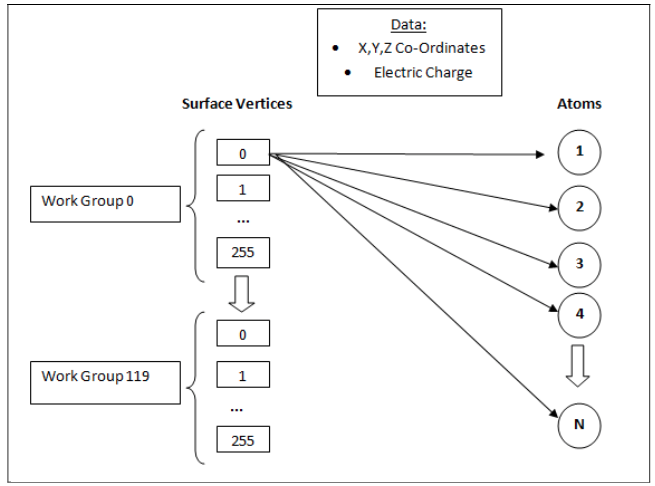
\includegraphics[width=0.5\textwidth]{figures/graph_nbody.png}
    \caption{Graphical representation of \emph{kernel} code.}
    \label{nbody_graph}
\end{figure}





